\documentclass[a4paper,11pt]{beamer}
\usepackage[utf8]{inputenc}
\usepackage{lmodern}
\usepackage{caption}
\usepackage{subcaption}
% Thème Darmstadt
\usetheme{Darmstadt}
\usepackage{graphicx}
\usepackage{ragged2e}
\usepackage{color}
\usepackage{booktabs}
\usepackage{tikz}
\usetikzlibrary{positioning, shapes.misc, calc}

%\captionsetup[figure]{labelformat=empty}

\setbeamertemplate{navigation symbols}{}
\setbeamertemplate{footline}
{
	\begin{beamercolorbox}[ht=2.5ex,dp=1.125ex,%
      leftskip=.3cm,rightskip=.3cm plus1fil]{title in head/foot}%
      {\usebeamerfont{title in head/foot}\insertshorttitle} \hfill
      \insertframenumber / \inserttotalframenumber%
    \end{beamercolorbox}%
}

% Informations sur la présentation
\title[ADAPOINT - Documentation technique]{Dispositif de pointage ADAPOINT\\Documentation technique}
\subtitle{Salle D109}
\author{}
\institute{Institut des Sciences du Mouvement}
\date{}

% Couleurs des types de liaisons (schémas de principe)
\definecolor{cSubD}{rgb}{0.10, 0.30, 0.65}     % câbles Sub-D (DB9, DB25, DB37)
\definecolor{cBanane}{rgb}{0.80, 0.10, 0.10}   % cordons à fiches bananes
\definecolor{cAlim}{rgb}{0.45, 0.45, 0.45}     % alimentations
\definecolor{cADU}{rgb}{0.85, 0.50, 0.00}      % liaison à définir ultérieurement
\definecolor{cTTL}{rgb}{0.12, 0.50, 0.20}      % signaux logiques ADwin

% Styles TikZ communs
\tikzset{
	appareil/.style={draw, rounded corners=2pt, fill=blue!8, align=center,
		font=\scriptsize\bfseries, minimum height=0.9cm, inner sep=3pt},
	maitre/.style={appareil, fill=yellow!25, very thick},
	passif/.style={appareil, fill=gray!12, font=\scriptsize},
	lien/.style={-latex, thick},
	num/.style={circle, draw=black, fill=white, text=black, inner sep=0.5pt, font=\tiny\bfseries, minimum size=3.6mm},
	etiq/.style={font=\tiny, align=center, fill=white, inner sep=1pt}
}
% Numéro de liaison
\newcommand{\lnum}[1]{\tikz[baseline=(n.base)]\node[num](n){#1};}

% Lien vers une documentation
\newcommand{\docref}[2]{\textcolor{blue}{\textbf{\underline{\href{#1}{#2}}}}}

%\includeonlyframes{current}

\begin{document}

% Première diapositive : Titre
\begin{frame}[plain]
    \titlepage
    \center{
\includegraphics[scale=0.75]{images/by-nc-sa.eps}}
 	\vspace{0.5cm}

	
\includegraphics[scale=0.6]{images/LogoAMU.png}\hspace*{2cm}
	
\includegraphics[scale=0.35]{images/LogoCNRS.eps}\hspace*{2cm}
	
\includegraphics[scale=0.09]{images/LogoISM.eps}

\end{frame}

\begin{frame}{Dispositif ADAPOINT}
	\tableofcontents[hideallsubsections]
\end{frame}

\AtBeginSection{%
    \begin{frame}
        \tableofcontents[sections=\value{section}]
    \end{frame}
}

%=====================================================================
\section{Présentation générale}
%=====================================================================
\subsection{Objet du document}
\begin{frame}
\justifying
Ce document décrit le poste expérimental de pointage \textbf{ADAPOINT} installé en salle D109. Il comporte deux parties :
\vspace{0.25cm}

\begin{block}{Les éléments du poste}
\justifying
Pour chaque élément : photographie et rôle dans le dispositif.
\end{block}

\begin{block}{Les liaisons filaires}
\justifying
Un schéma de principe global, puis le détail de chaque liaison : type de câble ou de connecteur (Sub-D DB9/DB25/DB37, fiches bananes...), numéros de broches et signaux transportés.
\end{block}
\vspace{0.25cm}

\centering
\textbf{\textcolor{red}{ADU = A Définir Ultérieurement}}
\end{frame}

\subsection{Vue d'ensemble}
\begin{frame}
\begin{block}{Les éléments du poste}
\begin{itemize}
	\item \textbf{ADwin-Gold-II} : système temps réel, élément de synchro.
	\item \textbf{CODAmotion / CodaHub (ODIN)} : mesures cinématiques
	\item \textbf{BIOPAC MP160} : mesures de l'activité musculaire (EMG)
	\item \textbf{Bouton poussoir à deux niveaux} : réponse du sujet
	\item \textbf{2 Cibles} (avec anneaux internes et externes)
	\begin{itemize}
		\item FarTarget
		\item ClosedTarget
	\end{itemize}
	\item \textbf{Boîtier relais photodiodes} : commande des cibles
	\item \textbf{Alimentation AL 841B} : alimentation 4,5V des cibles
	\item \textbf{Electro-aimant} pour position initiale
	\item \textbf{Boîtier relais} pour l'électro-aimant
	\item \textbf{Alimentation K.E.R.T.} : alimentation 4,5V \textbf{boîtier relais} et \textbf{électro-aimant}
\end{itemize}
\end{block}
\end{frame}

%=====================================================================
\section{Les éléments du poste}
%=====================================================================
\subsection{ADwin-Gold-II}
\begin{frame}{ADwin-Gold-II}
\begin{columns}[c]
\begin{column}{0.45\textwidth}
	\centering
	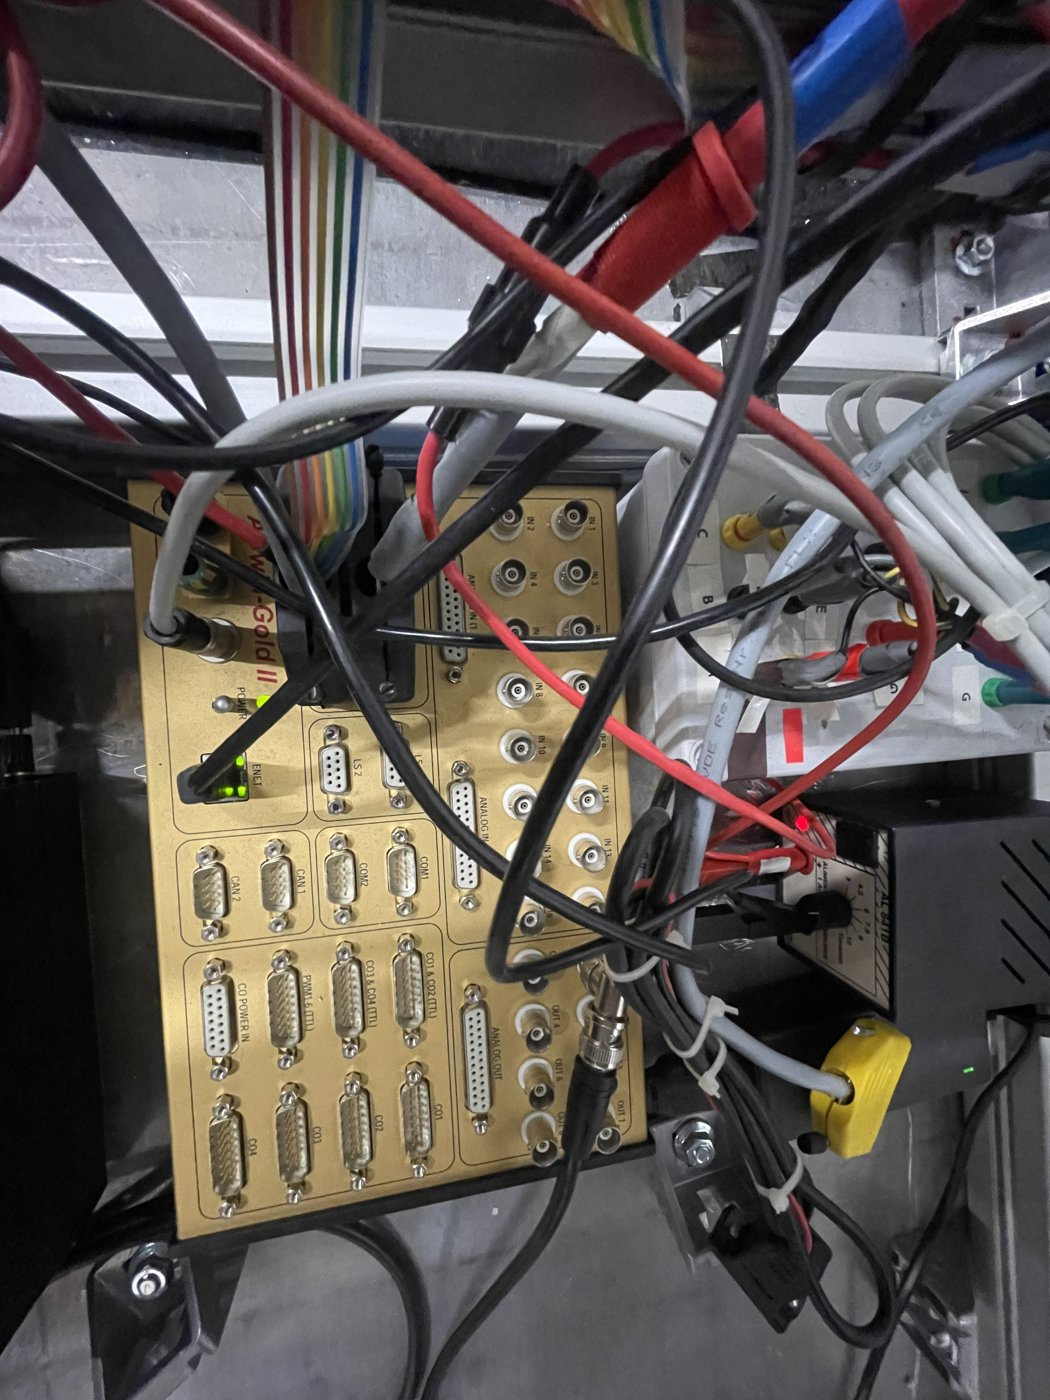
\includegraphics[height=0.7\textheight]{images/adwin_panneau.jpg}

	\scriptsize Panneau de connexion
\end{column}
\begin{column}{0.55\textwidth}
\begin{block}{Rôle}
\justifying
\footnotesize
Dispositif autonome et compact conçu pour l'acquisition de données et le contrôle en temps réel. C'est l'élément de synchronisation du poste :
\begin{itemize}
	\item lit le bouton poussoir
	\item allume les anneaux de LEDs des cibles
	\item commande l'électro-aimant
	\item déclenche les acquisitions CODA et BIOPAC (triggers)
	\item transmet des signaux analogiques au CODA et au BIOPAC
\end{itemize}
\end{block}
\end{column}
\end{columns}
\end{frame}

\begin{frame}{ADwin-Gold-II - Entrées / sorties digitales}
\begin{columns}[c]
\begin{column}{0.42\textwidth}
	\centering
	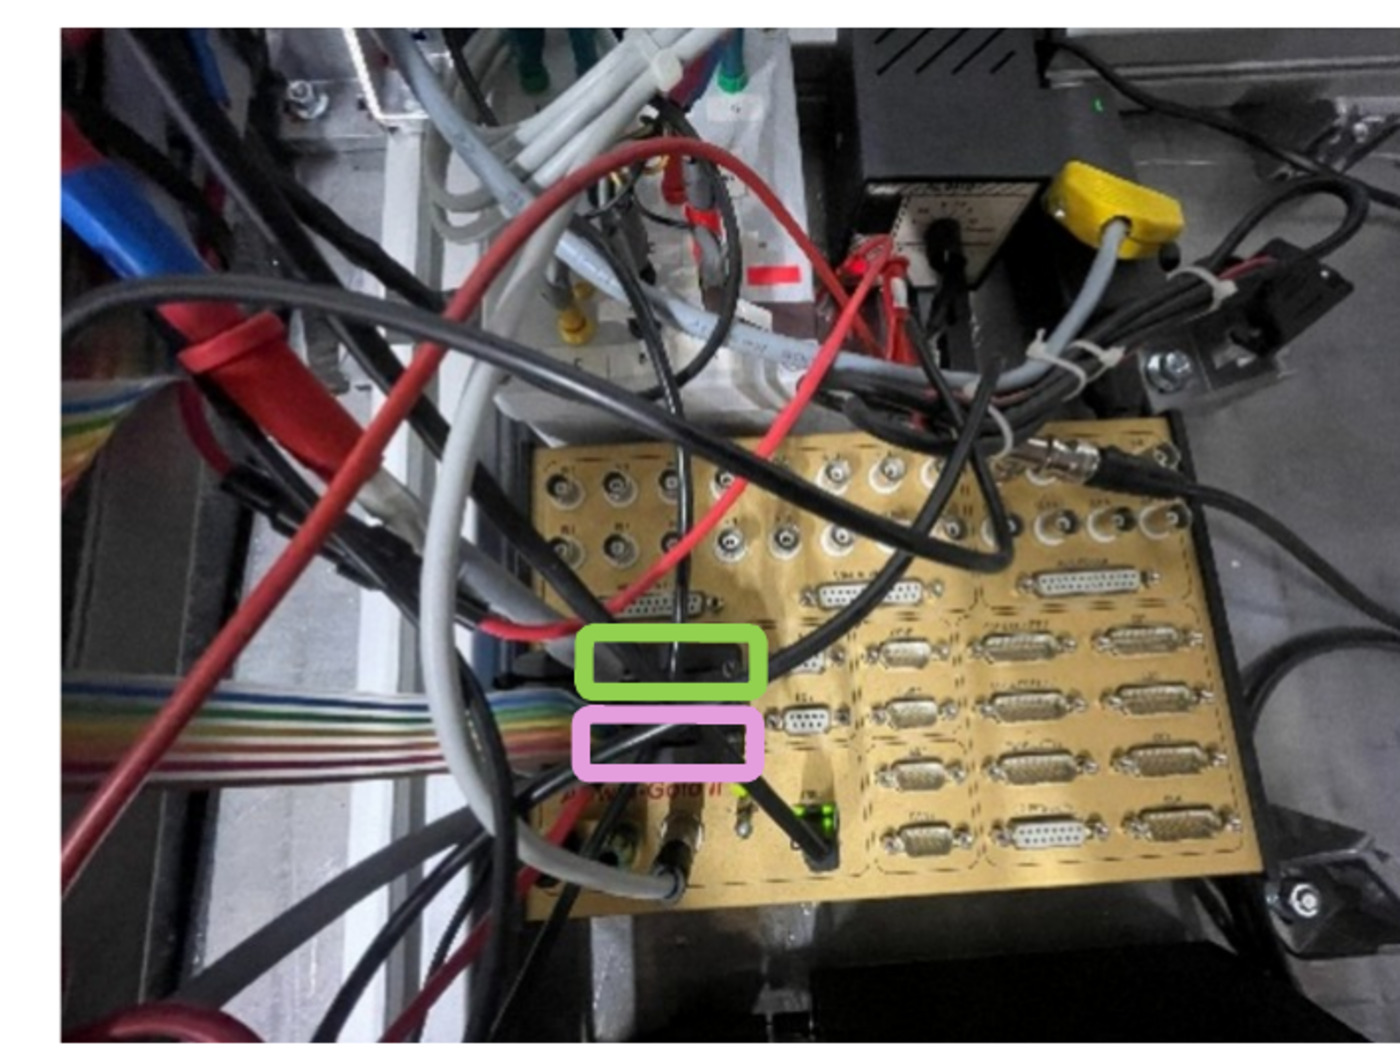
\includegraphics[width=\textwidth]{images/annot_adwin_dio.jpg}

	\scriptsize \textcolor{green!50!black}{\textbf{Vert}} : entrées digitales\\
	\textcolor{magenta}{\textbf{Rose}} : sorties digitales
\end{column}
\begin{column}{0.58\textwidth}
\begin{block}{Entrées digitales}
\scriptsize
\begin{itemize}
	\item Bit 0 : bouton poussoir niveau 1 (premier clic : pression faible)
	\item Bit 1 : bouton poussoir niveau 2 (deuxième clic : pression forte)
\end{itemize}
\end{block}
\begin{block}{Sorties digitales}
\scriptsize
\begin{itemize}
	\item Bit 0 : FarTarget External [FTE]
	\item Bit 1 : ClosedTarget External [CTE]
	\item Bit 2 : FarTarget Internal [FTI]
	\item Bit 3 : ClosedTarget Internal [CTI]
	\item Bit 4 : Trigger CODA
	\item Bit 5 : commande électro-aimant
	\item Bit 6 : Trigger BIOPAC
\end{itemize}
\end{block}
\end{column}
\end{columns}
\end{frame}

\subsection{CODAmotion / ODIN}
\begin{frame}{CODAmotion - CodaHub}
\begin{columns}[c]
\begin{column}{0.5\textwidth}
	\centering
	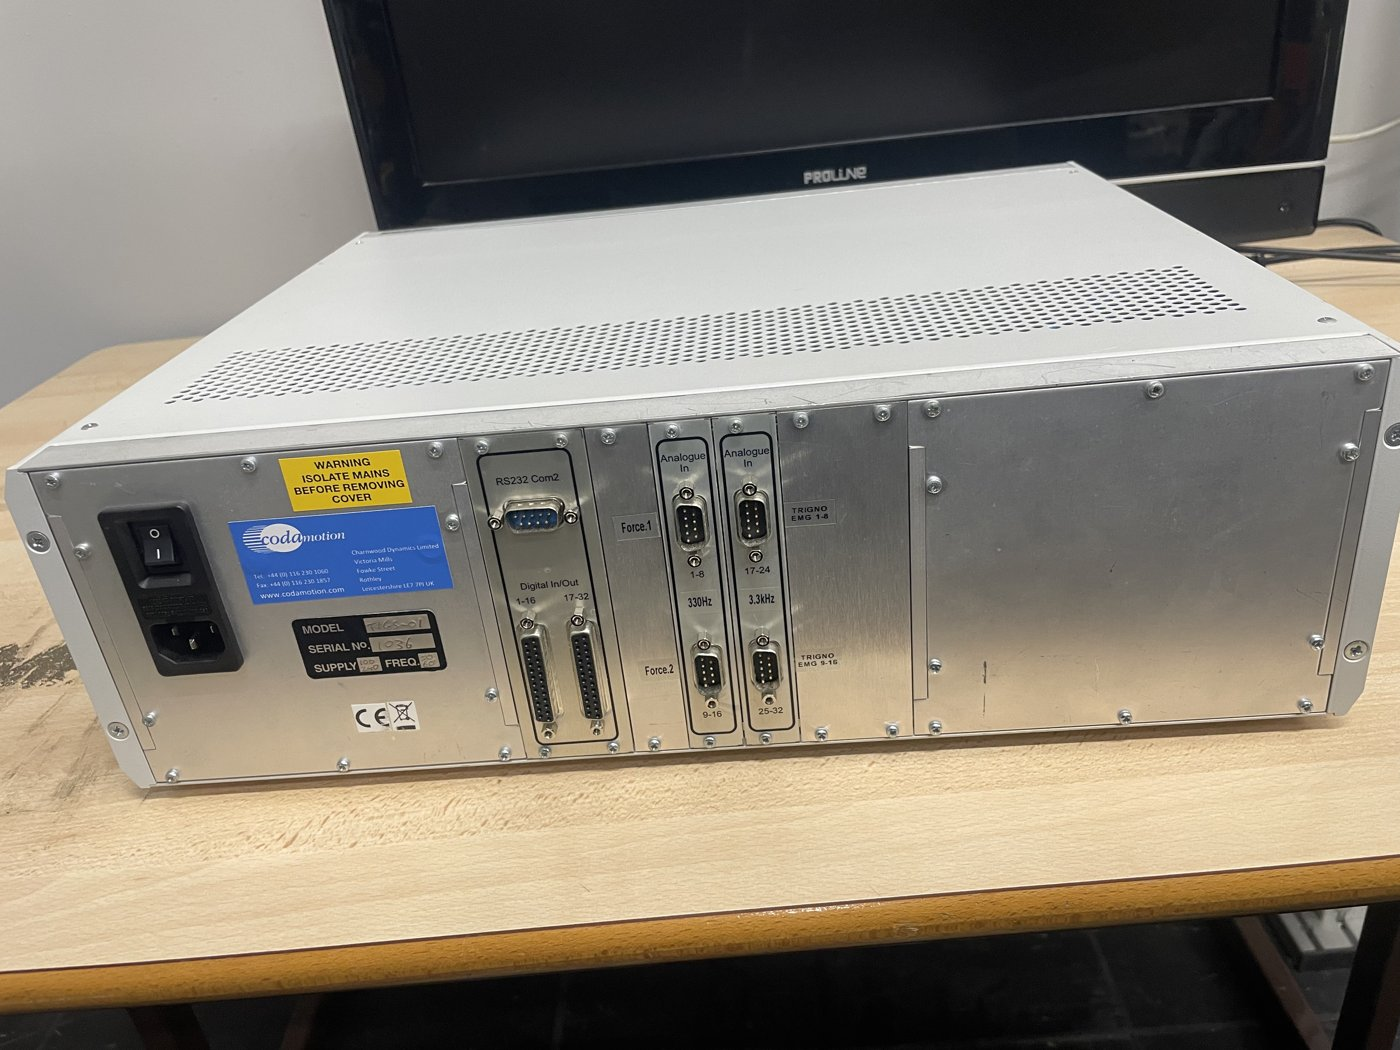
\includegraphics[width=0.85\textwidth]{images/codahub_arriere.jpg}

	\scriptsize Face arrière

	\vspace{0.1cm}
	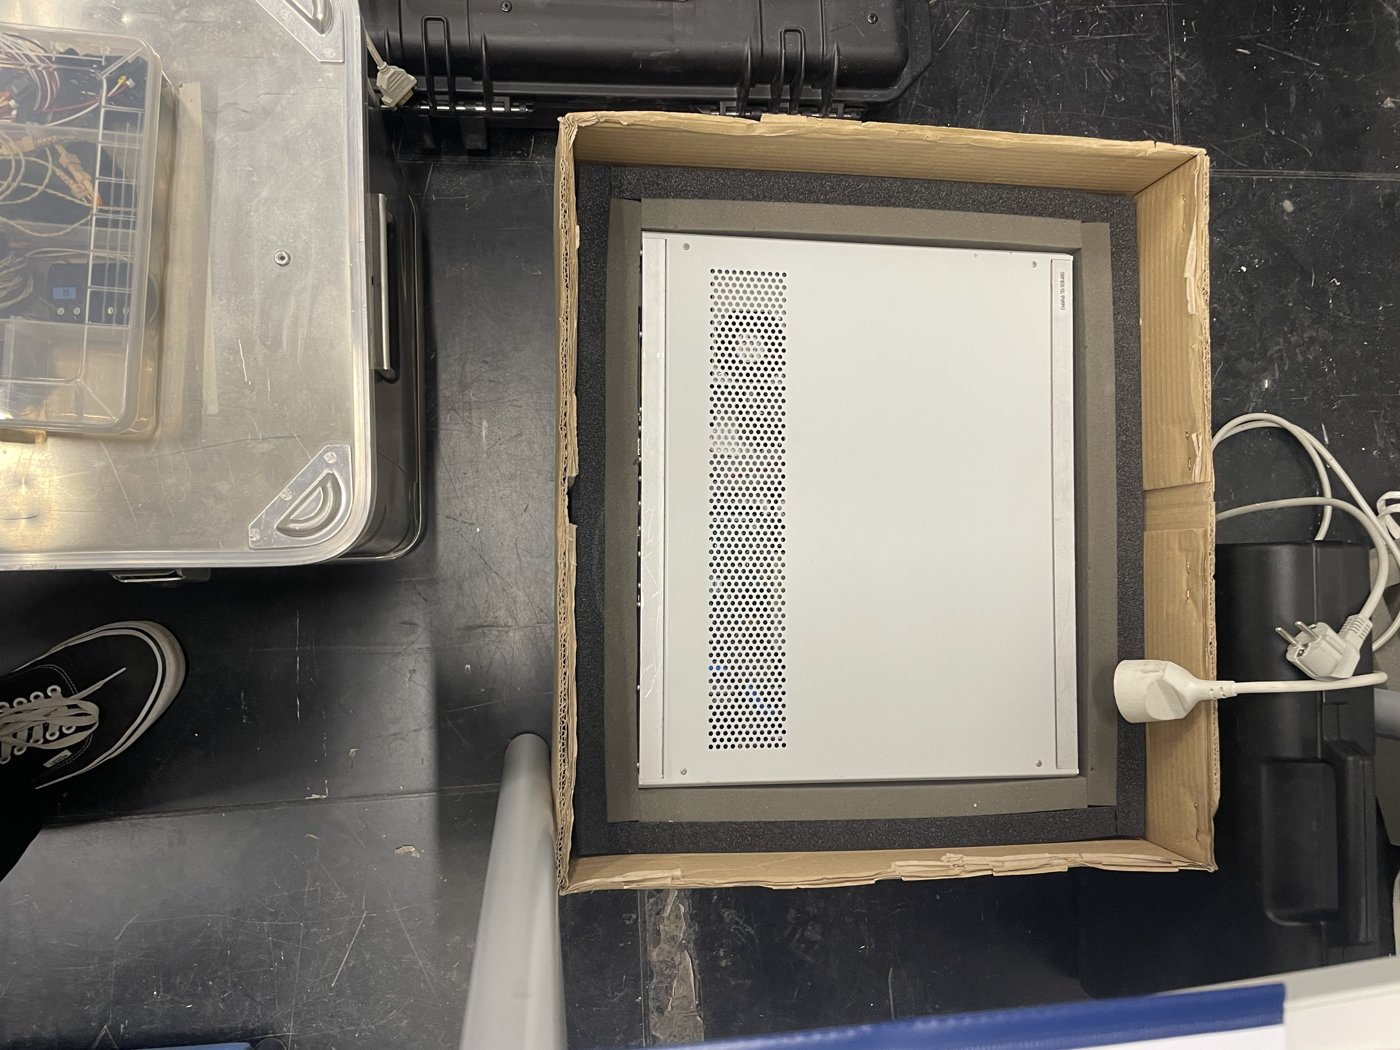
\includegraphics[width=0.5\textwidth]{images/codahub_dessus.jpg}

	\scriptsize Vue de dessus (CodaHub TIG-1036-AMU)
\end{column}
\begin{column}{0.5\textwidth}
\begin{block}{Rôle}
\justifying
\small
L'ensemble CODAmotion sert, grâce au logiciel \textbf{ODIN}, pour les \textbf{mesures cinématiques}.
\vspace{0.2cm}

Le CodaHub (modèle TIGS-01, n° de série 1036) centralise les acquisitions : il reçoit le trigger de démarrage de l'ADwin et dispose d'entrées analogiques synchronisées avec la capture du mouvement.
\end{block}
\end{column}
\end{columns}
\end{frame}

\begin{frame}{CODAmotion - Connecteurs de la face arrière}
\centering
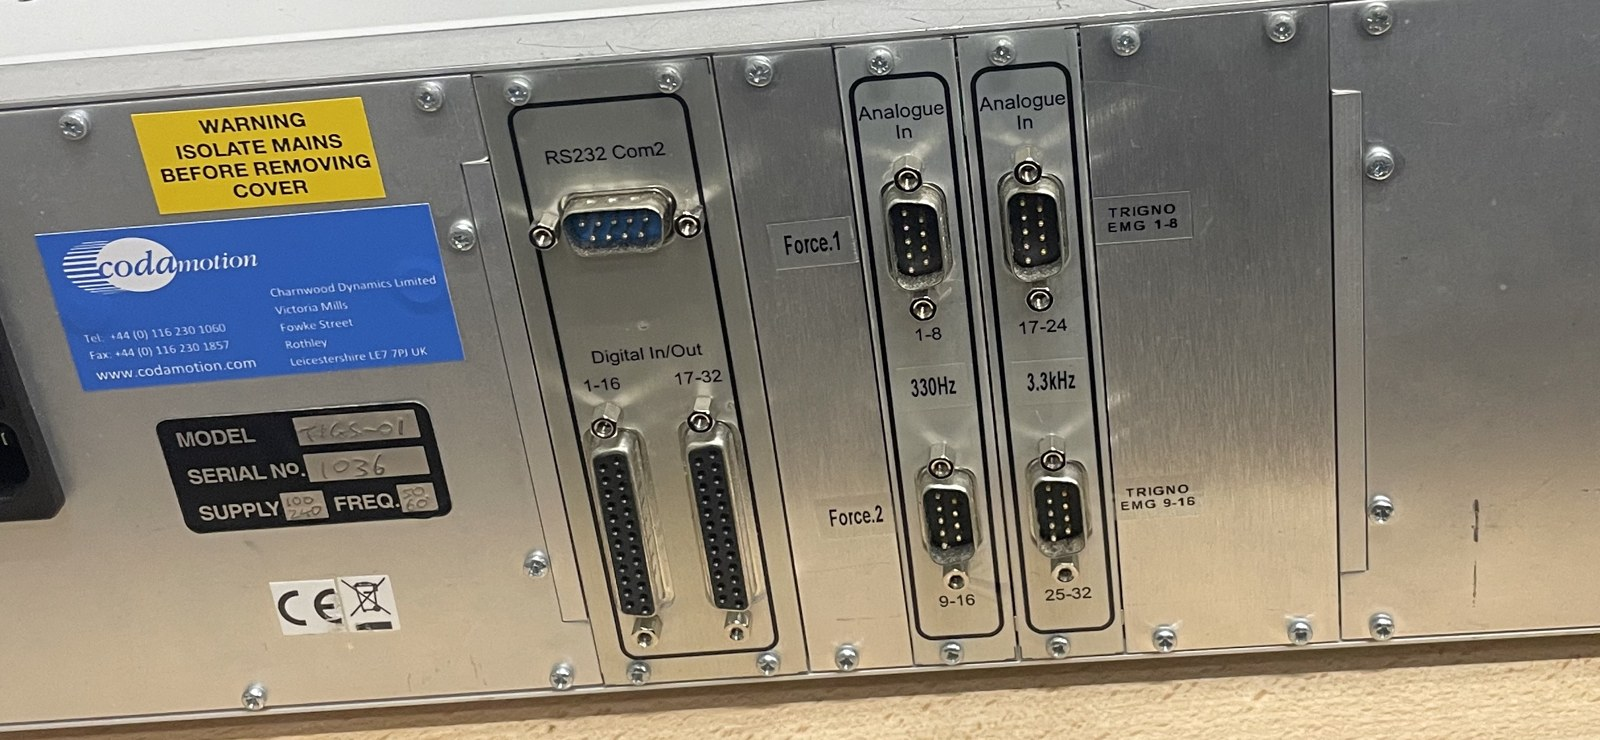
\includegraphics[width=0.9\textwidth]{images/codahub_connecteurs.jpg}
\vspace{0.1cm}

\scriptsize
\begin{tabular}{ll}
	\toprule
	\textbf{Connecteur} & \textbf{Fonction} \\
	\midrule
	DB9 (RS232 Com2) & liaison série \\
	2 $\times$ DB25 (Digital In/Out 1-16 et 17-32) & entrées/sorties logiques (trigger) \\
	4 $\times$ DB9 (Analogue In 1-8, 9-16 à 330Hz) & entrées analogiques \\
	\phantom{4 $\times$ DB9} (Analogue In 17-24, 25-32 à 3.3kHz) & \\
	\bottomrule
\end{tabular}
\end{frame}

\subsection{BIOPAC}
\begin{frame}{BIOPAC MP160}
\begin{columns}[c]
\begin{column}{0.5\textwidth}
	\centering
	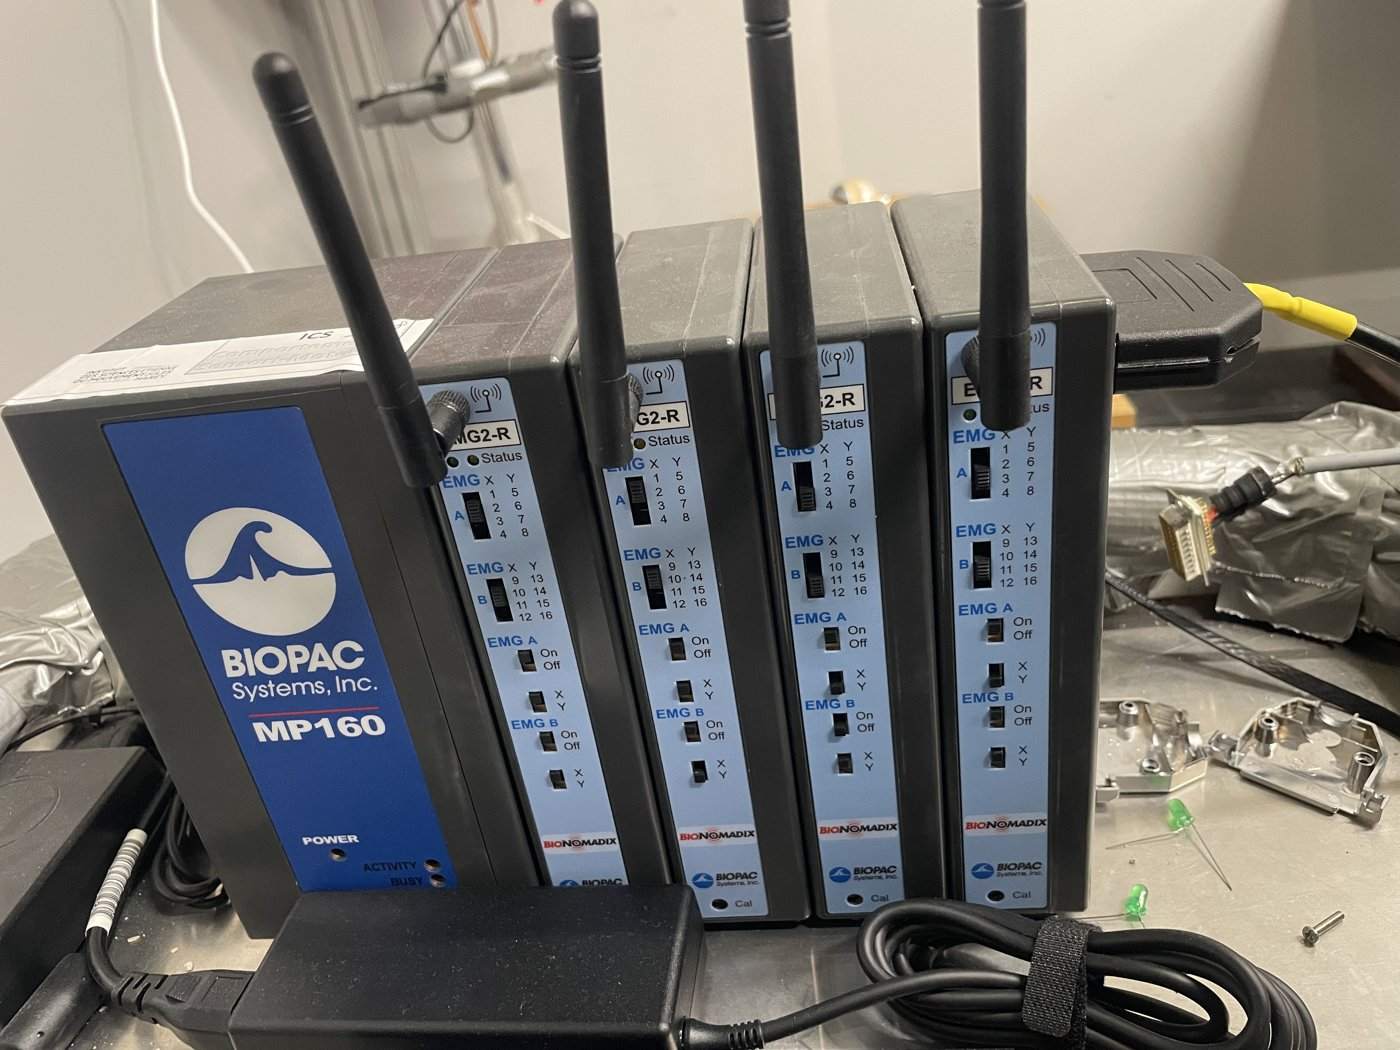
\includegraphics[width=\textwidth]{images/biopac_mp160.jpg}

	\scriptsize Unité MP160 et modules BioNomadix EMG2-R
\end{column}
\begin{column}{0.5\textwidth}
\begin{block}{Rôle}
\justifying
\small
L'ensemble BIOPAC sert pour les mesures de l'\textbf{activité musculaire (EMG)}.
\begin{itemize}
	\item MP160 : unité d'acquisition
	\item EMG2-R : récepteurs EMG sans fil (BioNomadix)
\end{itemize}
\vspace{0.2cm}
Il reçoit de l'ADwin un trigger externe et un signal analogique.
\end{block}
\end{column}
\end{columns}
\end{frame}

\subsection{Bouton poussoir et cibles}
\begin{frame}{Bouton poussoir et cibles}
\begin{block}{Bouton poussoir à deux niveaux}
\justifying
\small
Réponse du sujet. Un premier clic (pression faible) active le niveau 1, un deuxième clic (pression forte) le niveau 2. Chaque niveau est lu par une entrée digitale de l'ADwin (bits 0 et 1).
\end{block}
\begin{block}{Cibles}
\justifying
\small
Deux cibles, \textbf{FarTarget} (cible éloignée) et \textbf{ClosedTarget} (cible proche), possèdent chacune deux anneaux de LEDs :
\begin{itemize}
	\item un anneau externe (External) : FTE et CTE
	\item un anneau interne (Internal) : FTI et CTI
\end{itemize}
\end{block}
\centering
\textcolor{red}{\textbf{Photographies à compléter}}
\end{frame}

\subsection{Boîtier relais photodiodes}
\begin{frame}{Boîtier relais - Photodiodes}
\begin{columns}[c]
\begin{column}{0.42\textwidth}
	\centering
	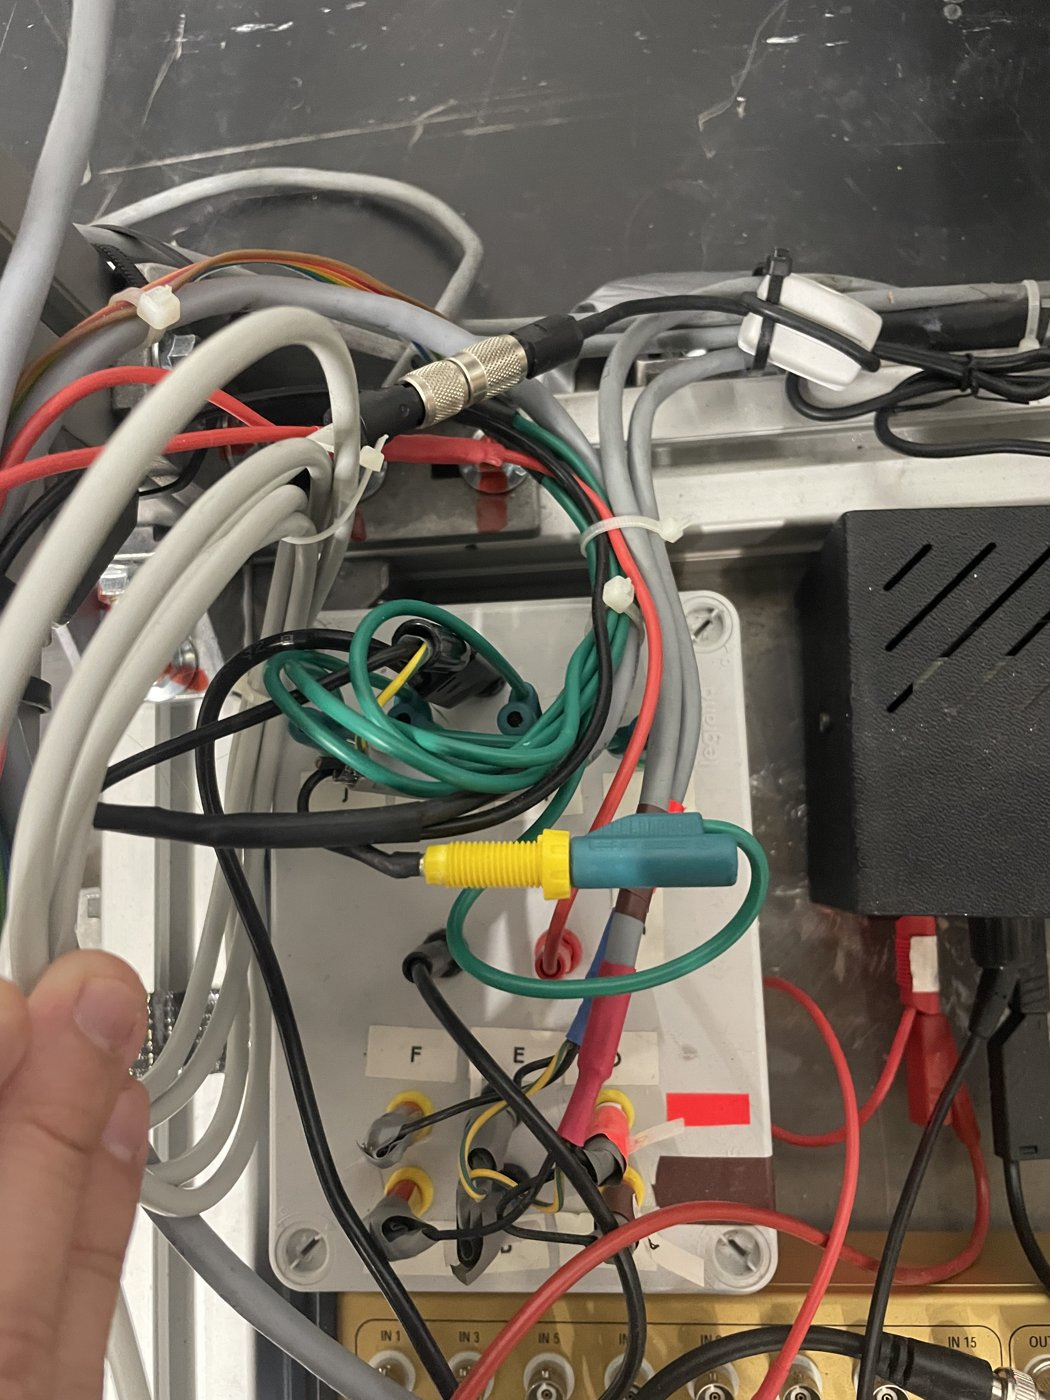
\includegraphics[height=0.72\textheight]{images/relais_photodiodes.jpg}
\end{column}
\begin{column}{0.58\textwidth}
\begin{block}{Rôle}
\justifying
\small
Interface de puissance entre les sorties digitales de l'ADwin (bits 0 à 3) et les quatre anneaux de LEDs des cibles.
\vspace{0.1cm}
\begin{itemize}
	\item 4 entrées de commande : G,H I et J
	\item 1 alimentation : GND et + (4,5V)
	\item 6 sorties : A, B, C (ClosedTarget) et D, E F (FarTarget)
\end{itemize}
\vspace{0.1cm}
Connexions par douilles bananes.
\end{block}
\end{column}
\end{columns}
\end{frame}

\subsection{Alimentation AL 841B}
\begin{frame}{Alimentation AL 841B}
\begin{columns}[c]
\begin{column}{0.5\textwidth}
	\centering
	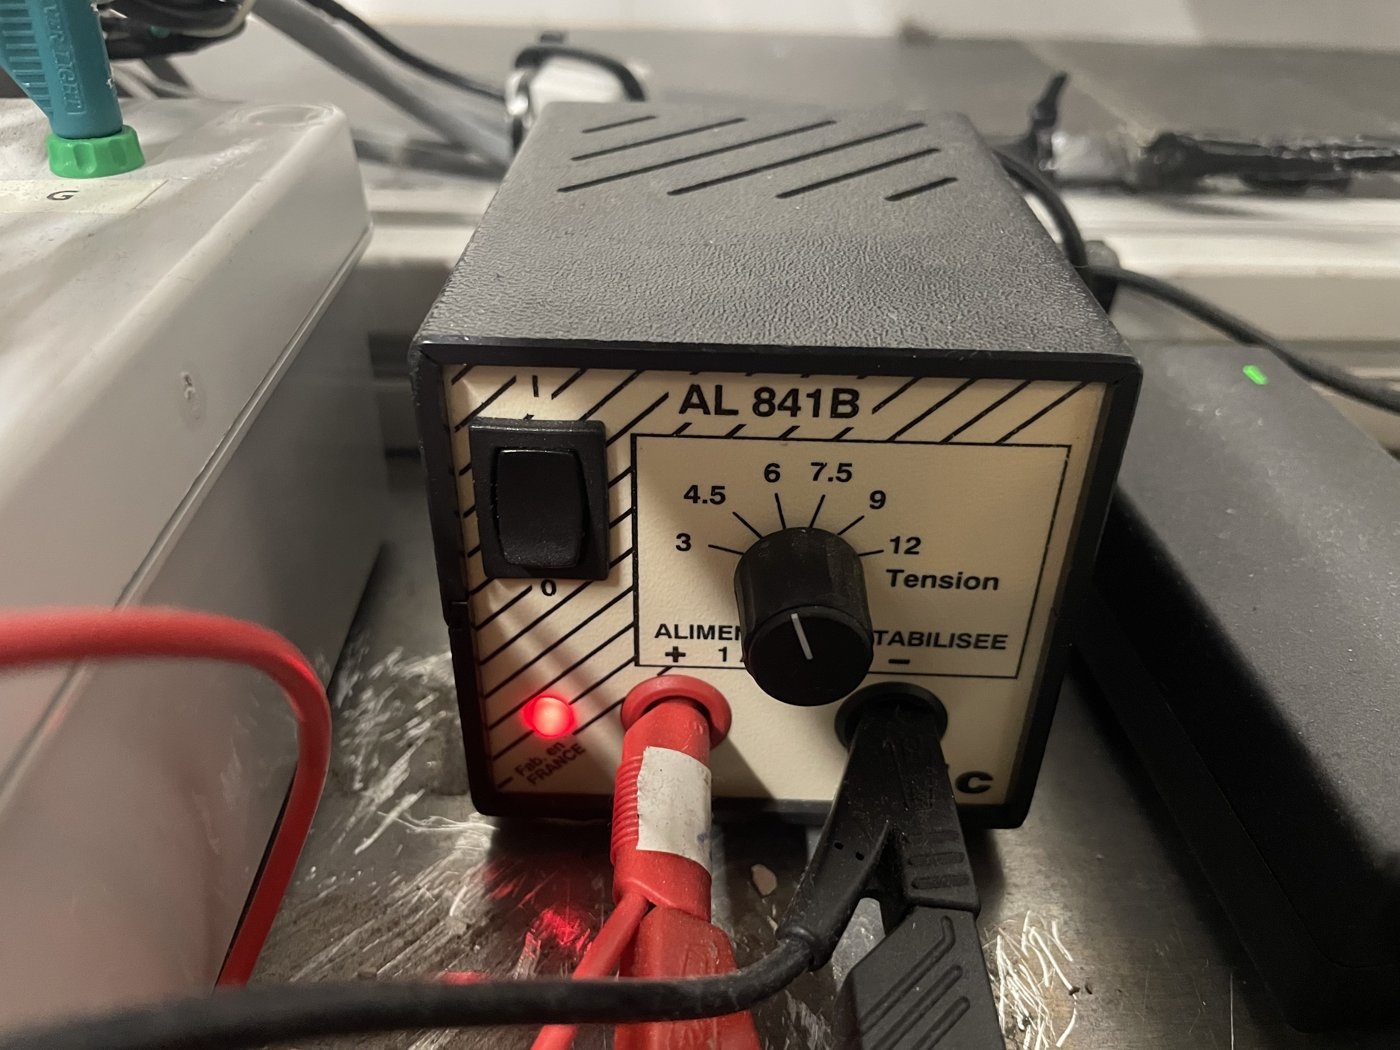
\includegraphics[width=\textwidth]{images/alim_al841b.jpg}
\end{column}
\begin{column}{0.5\textwidth}
\begin{block}{Rôle}
\justifying
\small
Alimentation stabilisée à tension réglable (3 à 12V par sélecteur).
\vspace{0.1cm}

Réglée sur \textbf{4.5V}, elle alimente les \textbf{LEDs des cibles} au travers du boîtier relais photodiodes (bornes GND et +). Sortie par cordons à fiches bananes (rouge : +, noir : $-$).
\end{block}
\end{column}
\end{columns}
\end{frame}

\subsection{Boîtier relais électro-aimant}
\begin{frame}{Boîtier relais - Électro-aimant}
\begin{columns}[c]
\begin{column}{0.42\textwidth}
	\centering
	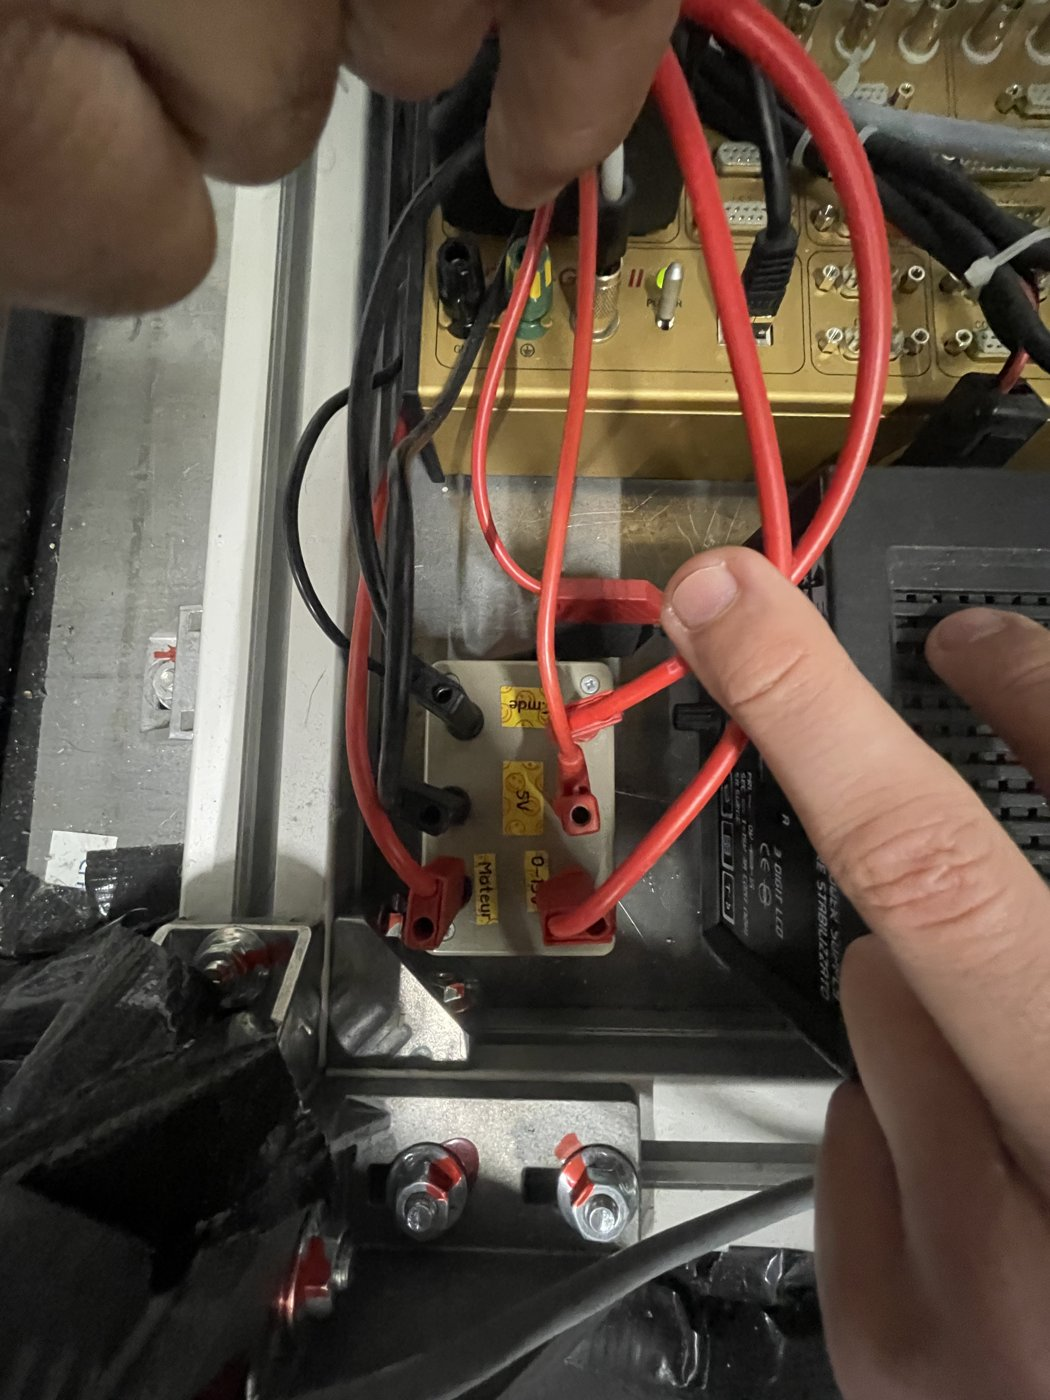
\includegraphics[height=0.72\textheight]{images/relais_electroaimant.jpg}
\end{column}
\begin{column}{0.58\textwidth}
\begin{block}{Rôle}
\justifying
\small
Petit boîtier à relais qui commute l'alimentation de l'électro-aimant sur ordre de l'ADwin (bit 5).
\vspace{0.1cm}
\begin{itemize}
	\item commande depuis l'ADwin (bit 5)
	\item 5V : alim. boîtier (AL 841B)
	\item 0-15V : alim. électro-aimant (KERT)
	\item "Moteur" : sortie relais vers électro-aimant
\end{itemize}
\vspace{0.1cm}
Connexions par douilles bananes.
\end{block}
\end{column}
\end{columns}
\end{frame}

\subsection{Alimentation K.E.R.T.}
\begin{frame}{Alimentation K.E.R.T.}
\begin{columns}[c]
\begin{column}{0.5\textwidth}
	\centering
	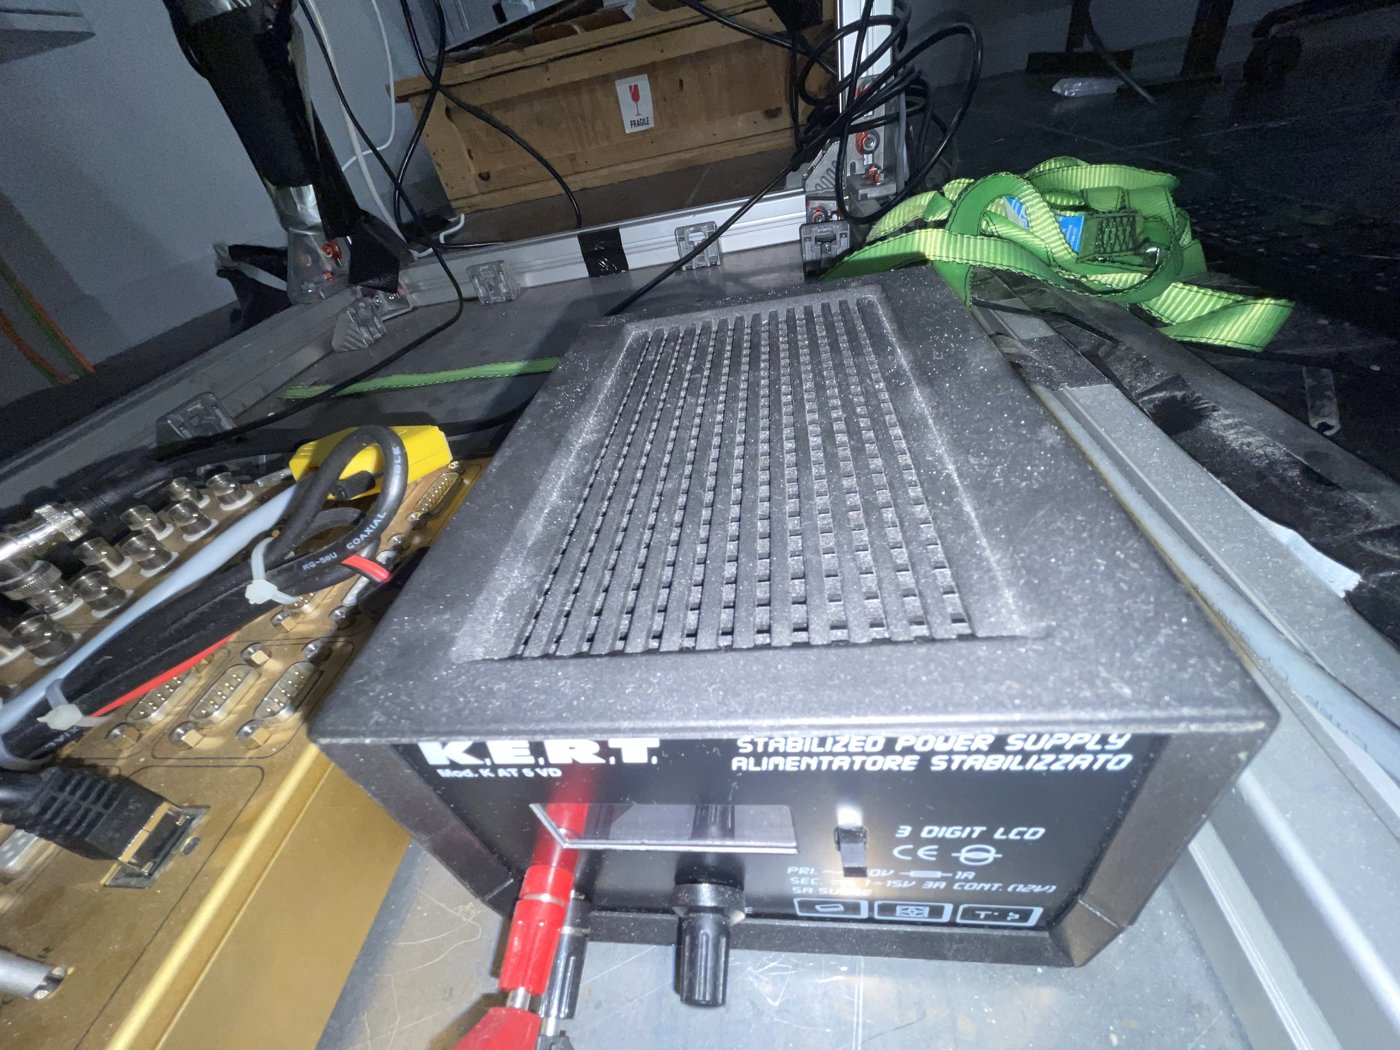
\includegraphics[width=\textwidth]{images/alim_kert.jpg}
\end{column}
\begin{column}{0.5\textwidth}
\begin{block}{Rôle}
\justifying
\small
Alimentation stabilisée (affichage LCD 2 digits).
\vspace{0.1cm}

Réglée sur \textbf{5V}, elle alimente la partie relais du \textbf{petit boîtier relais électro-aimant} (borne 0-15V).
\vspace{0.1cm}

Sortie par cordons à fiches bananes.
\end{block}
\end{column}
\end{columns}
\end{frame}

%=====================================================================
\section{Les liaisons filaires}
%=====================================================================
\subsection{Schéma de principe global}
\begin{frame}{Schéma de principe global}
\centering
\resizebox{\textwidth}{!}{%
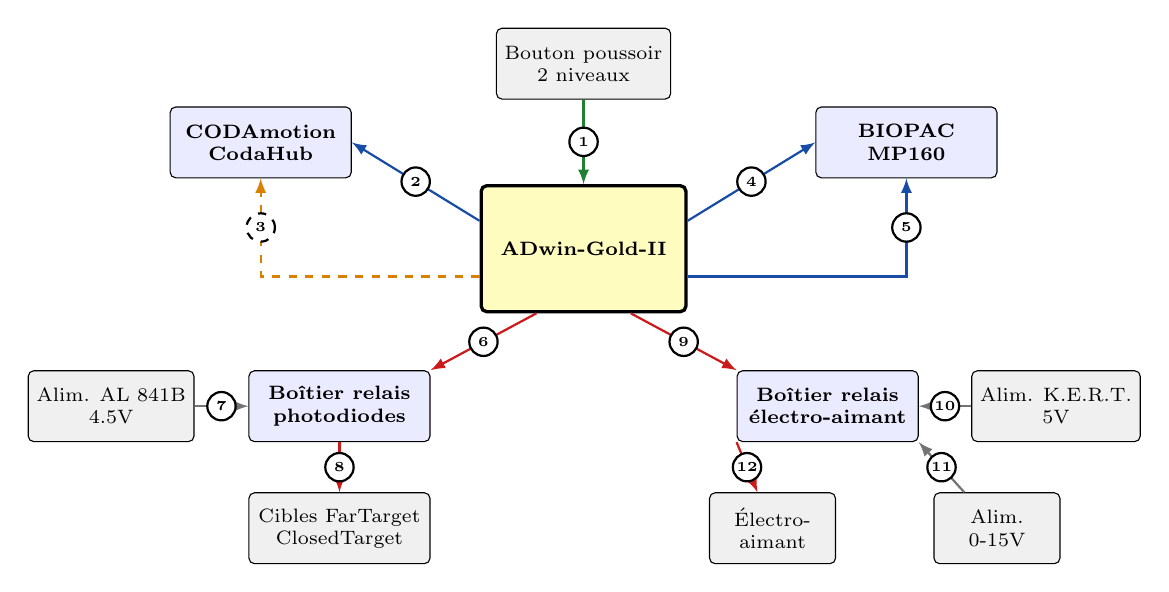
\begin{tikzpicture}[node distance=1cm]
	% Appareils
	\node[maitre, minimum width=2.6cm, minimum height=1.6cm] (adwin) at (0,0) {ADwin-Gold-II};
	\node[passif, minimum width=2.2cm] (bp) at (0,2.35) {Bouton poussoir\\2 niveaux};
	\node[appareil, minimum width=2.3cm] (coda) at (-4.1,1.35) {CODAmotion\\CodaHub};
	\node[appareil, minimum width=2.3cm] (biopac) at (4.1,1.35) {BIOPAC\\MP160};
	\node[appareil, minimum width=2.3cm] (rphoto) at (-3.1,-2.0) {Boîtier relais\\photodiodes};
	\node[passif, minimum width=1.8cm] (al841) at (-6.0,-2.0) {Alim. AL 841B\\4.5V};
	\node[passif, minimum width=2.3cm] (cibles) at (-3.1,-3.55) {Cibles FarTarget\\ClosedTarget};
	\node[appareil, minimum width=2.3cm] (relec) at (3.1,-2.0) {Boîtier relais\\électro-aimant};
	\node[passif, minimum width=1.8cm] (kert) at (6.0,-2.0) {Alim. K.E.R.T.\\5V};
	\node[passif, minimum width=1.6cm] (alim15) at (5.25,-3.55) {Alim.\\0-15V};
	\node[passif, minimum width=1.6cm] (ea) at (2.4,-3.55) {Électro-\\aimant};

	% Liaisons
	\draw[lien, cTTL] (bp) -- node[num, pos=0.5]{1} (adwin);
	\draw[lien, cSubD] (adwin.165) -- node[num, pos=0.5]{2} (coda.east);
	\draw[lien, cADU, dashed] (adwin.195) -| node[num, pos=0.75]{3} (coda.south);
	\draw[lien, cSubD] (adwin.15) -- node[num, pos=0.5]{4} (biopac.west);
	\draw[lien, cSubD] (adwin.-15) -| node[num, pos=0.75]{5} (biopac.south);
	\draw[lien, cBanane] ([xshift=-6mm]adwin.south) -- node[num, pos=0.5]{6} (rphoto.north east);
	\draw[lien, cAlim] (al841) -- node[num, pos=0.5]{7} (rphoto);
	\draw[lien, cBanane] (rphoto) -- node[num, pos=0.5]{8} (cibles);
	\draw[lien, cBanane] ([xshift=6mm]adwin.south) -- node[num, pos=0.5]{9} (relec.north west);
	\draw[lien, cAlim] (kert) -- node[num, pos=0.5]{10} (relec);
	\draw[lien, cAlim] (alim15) -- node[num, pos=0.5]{11} (relec.south east);
	\draw[lien, cBanane] (relec.south west) -- node[num, pos=0.5]{12} (ea);
\end{tikzpicture}}

\vspace{0.1cm}
\tiny
\textcolor{cSubD}{\rule{4mm}{1pt}} câble Sub-D \quad
\textcolor{cBanane}{\rule{4mm}{1pt}} banane (signal) \quad
\textcolor{cAlim}{\rule{4mm}{1pt}} banane (alim.) \quad
\textcolor{cTTL}{\rule{4mm}{1pt}} entrée logique \quad
\textcolor{cADU}{- - -} ADU
\end{frame}

\subsection{Tableau récapitulatif}
\begin{frame}{Tableau récapitulatif des liaisons}
\centering
\tiny
\setlength{\tabcolsep}{3pt}
\begin{tabular}{clllp{3.6cm}}
	\toprule
	\textbf{N°} & \textbf{De} & \textbf{Vers} & \textbf{Câble / connecteur} & \textbf{Signaux} \\
	\midrule
	1  & Bouton poussoir   & ADwin (DI)          & Câble classique                 & Bits 0 et 1 : niveaux 1 et 2 \\
	2  & ADwin (DO)        & CODA                & DB25 (jaune)        & Bit 4 : Trigger CODA, broches 22, 23 \\
	3  & ADwin             & CODA                & DB9 (noir)          & ADU (nécessite ODIN) \\
	4  & ADwin (AO)        & BIOPAC              & DB37 (orange clair) & Canal analogique n°6 \\
	5  & ADwin (DO)        & BIOPAC              & DB25 (bleu clair)   & Bit 6 : external trigger \\
	6  & ADwin (DO)        & Relais photodiodes  & Bananes             & Bits 0 à 3 $\rightarrow$ G, H, I, J \\
	7  & Alim. AL 841B     & Relais photodiodes  & Bananes             & 4,5V : GND et + \\
	8  & Relais photodiodes& Cibles              & Bananes             & A, B, C et D, E, F \\
	9  & ADwin (DO)        & Relais électro-aimant & Bananes           & Bit 5 $\rightarrow$ Cmde \\
	10 & Alim. AL814B    & Relais électro-aimant & Bananes           & 4,5V $\rightarrow$ 5V \\
	11 & Alim. K.E.R.T.       & Electro-aimant & Bananes           & 0-15V \\
	12 & Relais électro-aimant & Électro-aimant  & Bananes             & Sortie "Moteur" \\
	\bottomrule
\end{tabular}
\vspace{0.3cm}

\scriptsize
DI / DO : entrées / sorties digitales -- AO : sorties analogiques
\end{frame}

%---------------------------------------------------------------------
\subsection{ADwin $\leftrightarrow$ CODAmotion}
\begin{frame}{Liaisons \lnum{2} et \lnum{3} : ADwin $\rightarrow$ CODAmotion}
\begin{columns}[c]
\begin{column}{0.5\textwidth}
	\centering
	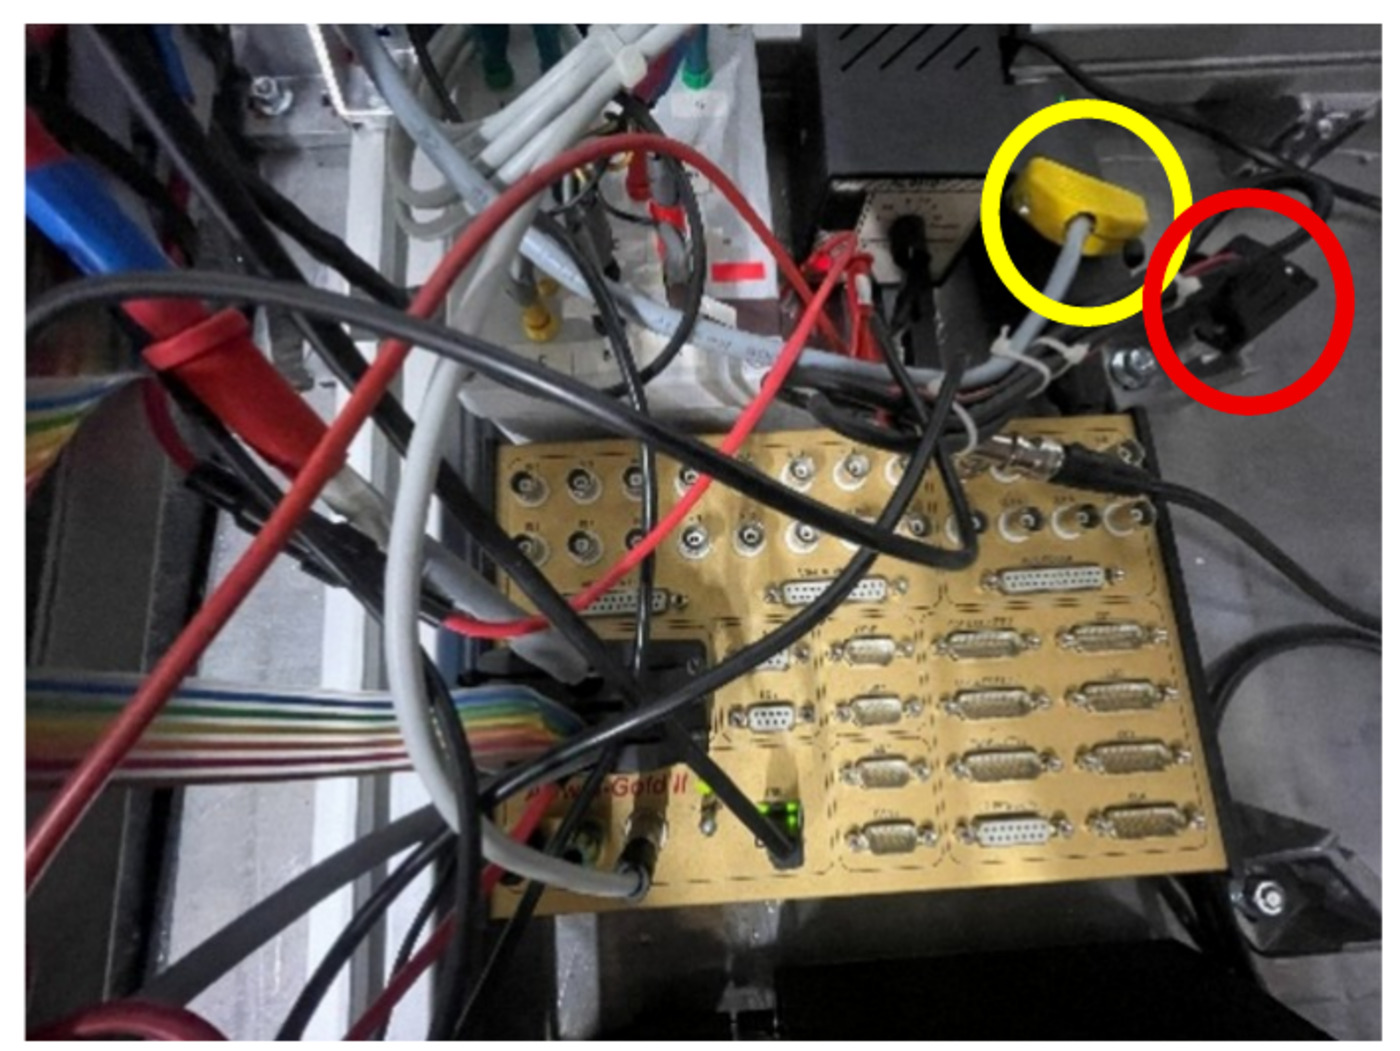
\includegraphics[width=\textwidth]{images/annot_adwin_coda.jpg}

	\scriptsize Côté ADwin
\end{column}
\begin{column}{0.5\textwidth}
	\centering
	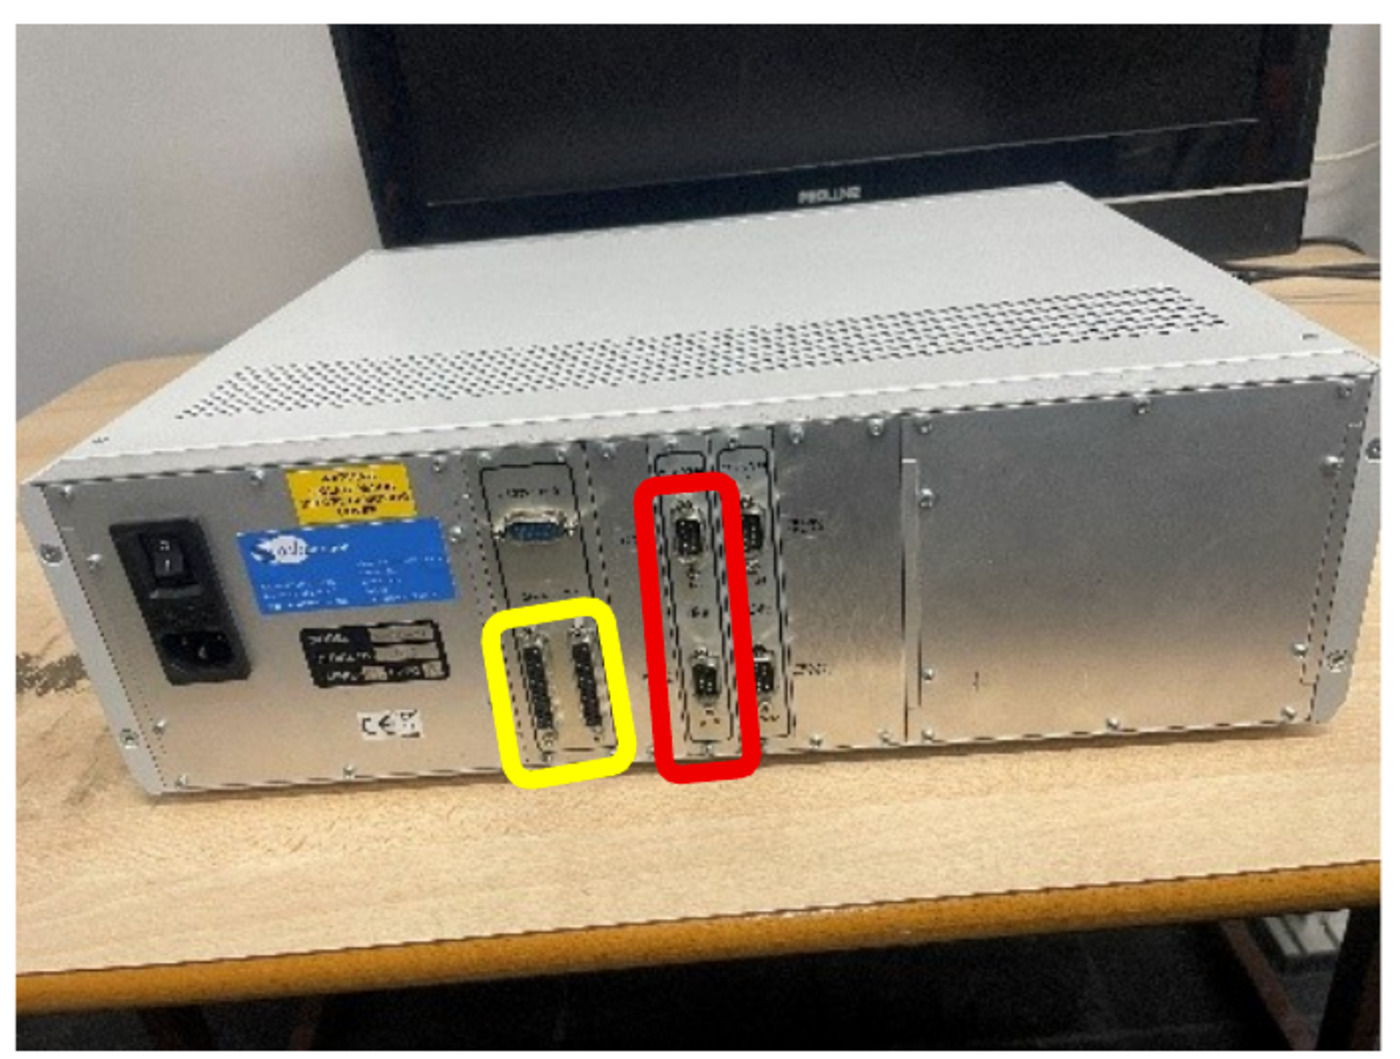
\includegraphics[width=\textwidth]{images/annot_coda.jpg}

	\scriptsize Côté CodaHub
\end{column}
\end{columns}
\vspace{0.2cm}
\justifying
\small
Côté CodaHub, chaque câble se connectera sur l'un des deux emplacements encadrés de la même couleur (\textcolor{red}{\textbf{ADU}}) :
\begin{itemize}
	\item \textcolor{yellow!60!black}{\textbf{Jaune}} : DB25 Digital In/Out 1-16 ou 17-32
	\item \textcolor{red}{\textbf{Rouge}} : DB9 Analogue In 1-8 ou 9-16
\end{itemize}
\end{frame}

\begin{frame}{Liaisons \lnum{2} et \lnum{3} : brochages}
\begin{columns}[t]
\begin{column}{0.5\textwidth}
\begin{block}{\lnum{2} Trigger CODAmotion - DB25}
\small
Connecteur jaune (entouré en jaune)
\vspace{0.1cm}

\centering
\begin{tabular}{cl}
	\toprule
	\textbf{Broche} & \textbf{Signal} \\
	\midrule
	22 & Start Acquisition \\
	23 & Masse (GND) \\
	\bottomrule
\end{tabular}
\vspace{0.1cm}

\justifying
\scriptsize
Signal issu de la sortie digitale bit 4 (Trigger CODA) de l'ADwin.
\end{block}
\end{column}
\begin{column}{0.5\textwidth}
\begin{block}{\lnum{3} Liaison ODIN - DB9}
\small
Connecteur noir (entouré en rouge)
\vspace{0.1cm}

\centering
\begin{tabular}{cl}
	\toprule
	\textbf{Broche} & \textbf{Signal} \\
	\midrule
	ADU & ADU \\
	\bottomrule
\end{tabular}
\vspace{0.1cm}

\justifying
\scriptsize
Nécessite ODIN : brochage à établir à partir de la documentation CODAmotion.
\end{block}
\end{column}
\end{columns}
\vspace{0.3cm}

\centering
\textcolor{red}{\textbf{Regarder dans la documentation ODIN}}
\end{frame}

%---------------------------------------------------------------------
\subsection{ADwin $\leftrightarrow$ BIOPAC}
\begin{frame}{Liaisons \lnum{4} et \lnum{5} : ADwin $\rightarrow$ BIOPAC}
\begin{columns}[c]
\begin{column}{0.5\textwidth}
	\centering
	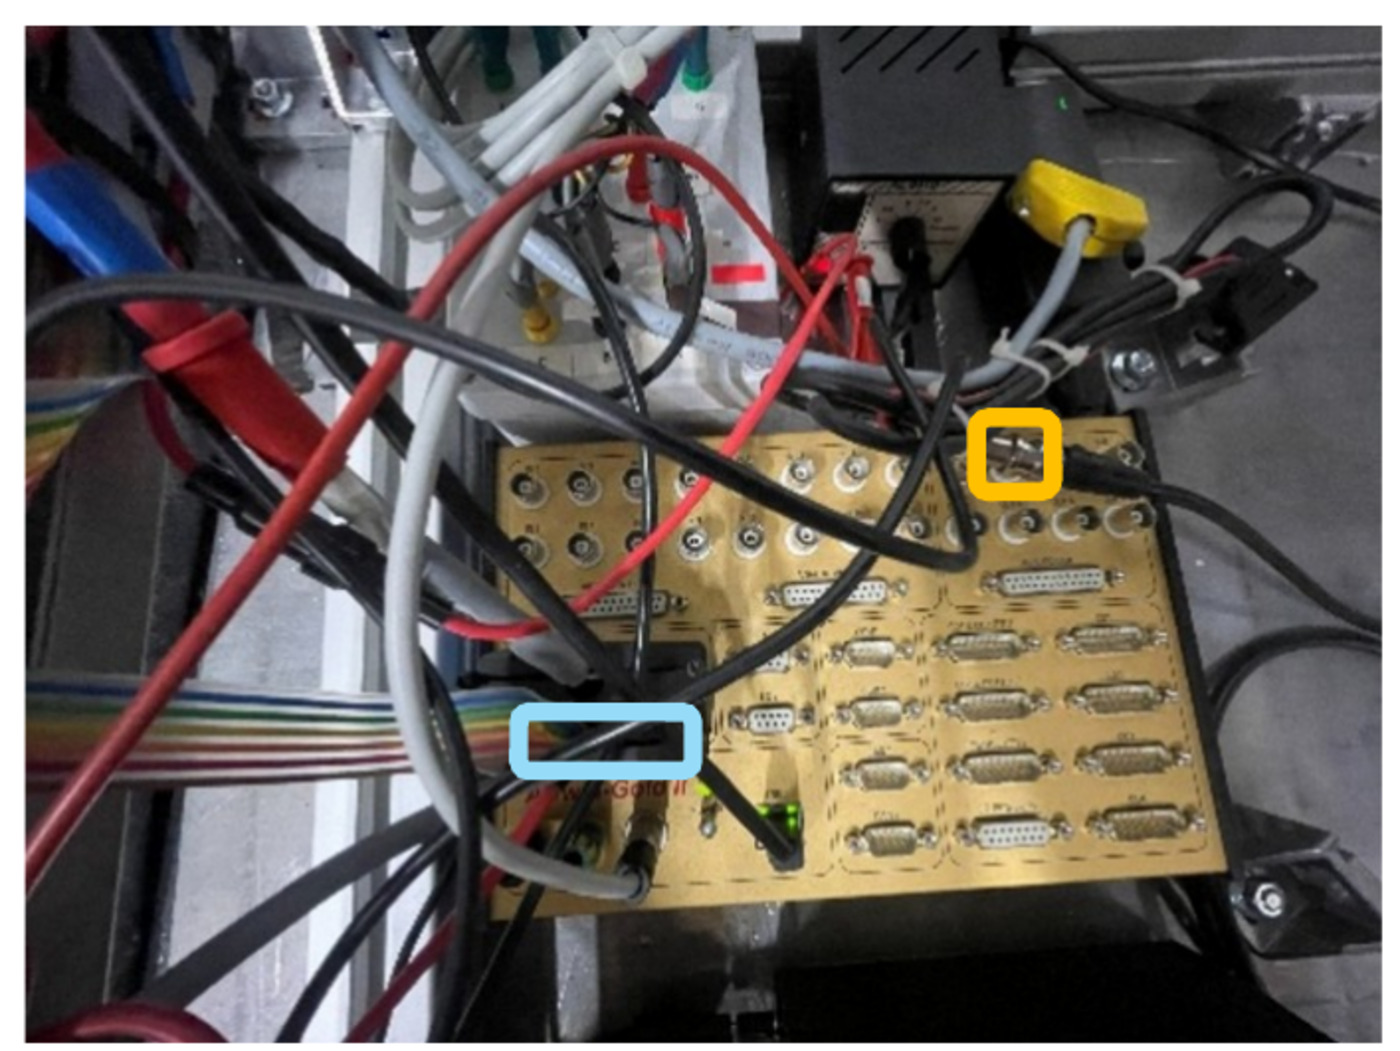
\includegraphics[width=\textwidth]{images/annot_adwin_biopac.jpg}

	\scriptsize Côté ADwin
\end{column}
\begin{column}{0.5\textwidth}
	\centering
	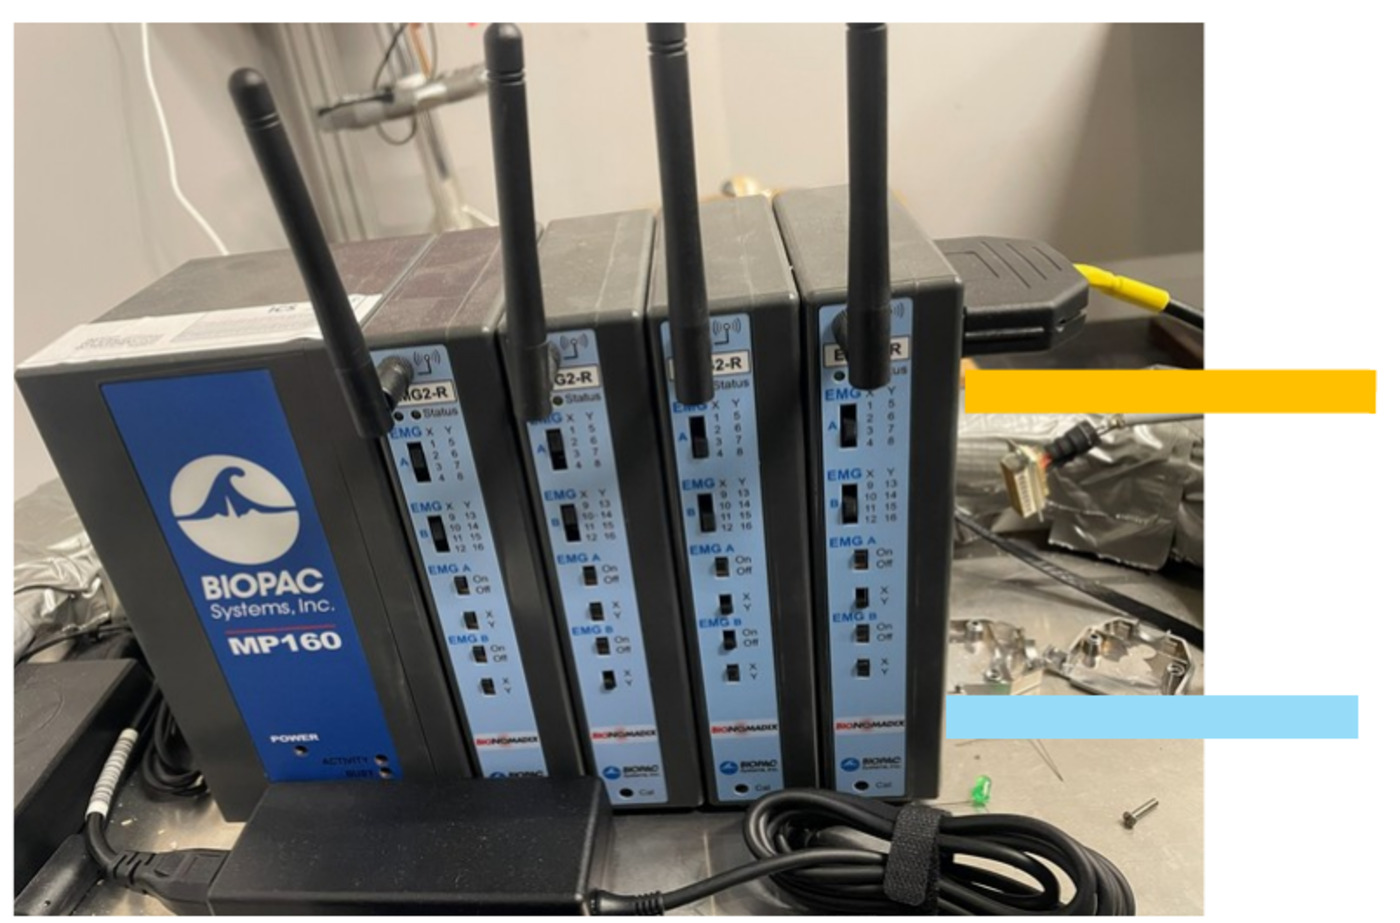
\includegraphics[width=\textwidth]{images/annot_biopac.jpg}

	\scriptsize Côté BIOPAC (flanc droit)
\end{column}
\end{columns}
\vspace{0.2cm}
\small
\begin{itemize}
	\item \textcolor{orange}{\textbf{Orange clair}} : DB37, flanc droit en haut du BIOPAC
	\item \textcolor{cyan!70!black}{\textbf{Bleu clair}} : DB25, flanc droit en bas du BIOPAC
\end{itemize}
\end{frame}

\begin{frame}{Liaisons \lnum{4} et \lnum{5} : brochages}
\begin{columns}[t]
\begin{column}{0.5\textwidth}
\begin{block}{\lnum{4} Entrées analogiques - DB37}
\scriptsize
ADwin : sorties analogiques\\
BIOPAC : flanc droit, en haut
\vspace{0.1cm}

\centering
\small
\begin{tabular}{cl}
	\toprule
	\textbf{Broche} & \textbf{Signal} \\
	\midrule
	1  & Masse (GND) \\
	25 & Canal analogique n°6 \\
	\bottomrule
\end{tabular}
\end{block}
\end{column}
\begin{column}{0.5\textwidth}
\begin{block}{\lnum{5} E/S digitales - DB25}
\scriptsize
ADwin : sorties digitales (bit 6)\\
BIOPAC : flanc droit, en bas
\vspace{0.1cm}

\centering
\small
\begin{tabular}{cl}
	\toprule
	\textbf{Broche} & \textbf{Signal} \\
	\midrule
	5 et 6 & Masse (GND) \\
	7      & External trigger \\
	\bottomrule
\end{tabular}
\end{block}
\end{column}
\end{columns}
\end{frame}

%---------------------------------------------------------------------
\subsection{Bouton poussoir $\rightarrow$ ADwin}
\begin{frame}{Liaison \lnum{1} : bouton poussoir $\rightarrow$ ADwin}
\centering
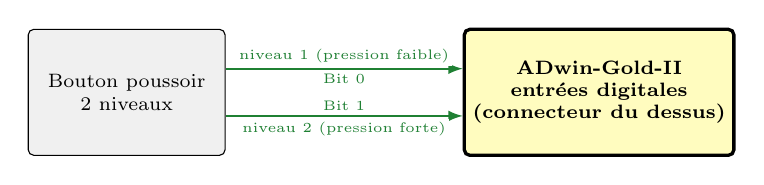
\begin{tikzpicture}
	\node[passif, minimum width=2.5cm, minimum height=1.6cm] (bp) at (0,0) {Bouton poussoir\\2 niveaux};
	\node[maitre, minimum width=3.4cm, minimum height=1.6cm] (adwin) at (6,0) {ADwin-Gold-II\\\scriptsize entrées digitales\\\scriptsize(connecteur du dessus)};
	\draw[lien, cTTL] ([yshift=3mm]bp.east) -- node[etiq, above=0.25mm]{niveau 1 (pression faible)} node[etiq, below=0.25mm]{Bit 0} ([yshift=3mm]adwin.west);
	\draw[lien, cTTL] ([yshift=-3mm]bp.east) -- node[etiq, below=0.25mm, 
	]{niveau 2 (pression forte)} node[etiq, above=0.25mm]{Bit 1} ([yshift=-3mm]adwin.west);
\end{tikzpicture}
\vspace{0.5cm}

\begin{table}
\small
\begin{tabular}{lll}
	\toprule
	\textbf{Signal} & \textbf{Entrée ADwin} & \textbf{Broche} \\
	\midrule
	Niveau 1 (premier clic)  & DI Bit 0 & ADU \\
	Niveau 2 (deuxième clic) & DI Bit 1 & ADU \\
	\bottomrule
\end{tabular}
\end{table}
\end{frame}

%---------------------------------------------------------------------
\subsection{Commande des cibles}
\begin{frame}{Liaisons \lnum{6}, \lnum{7} et \lnum{8} : boîtier relais photodiodes}
\centering
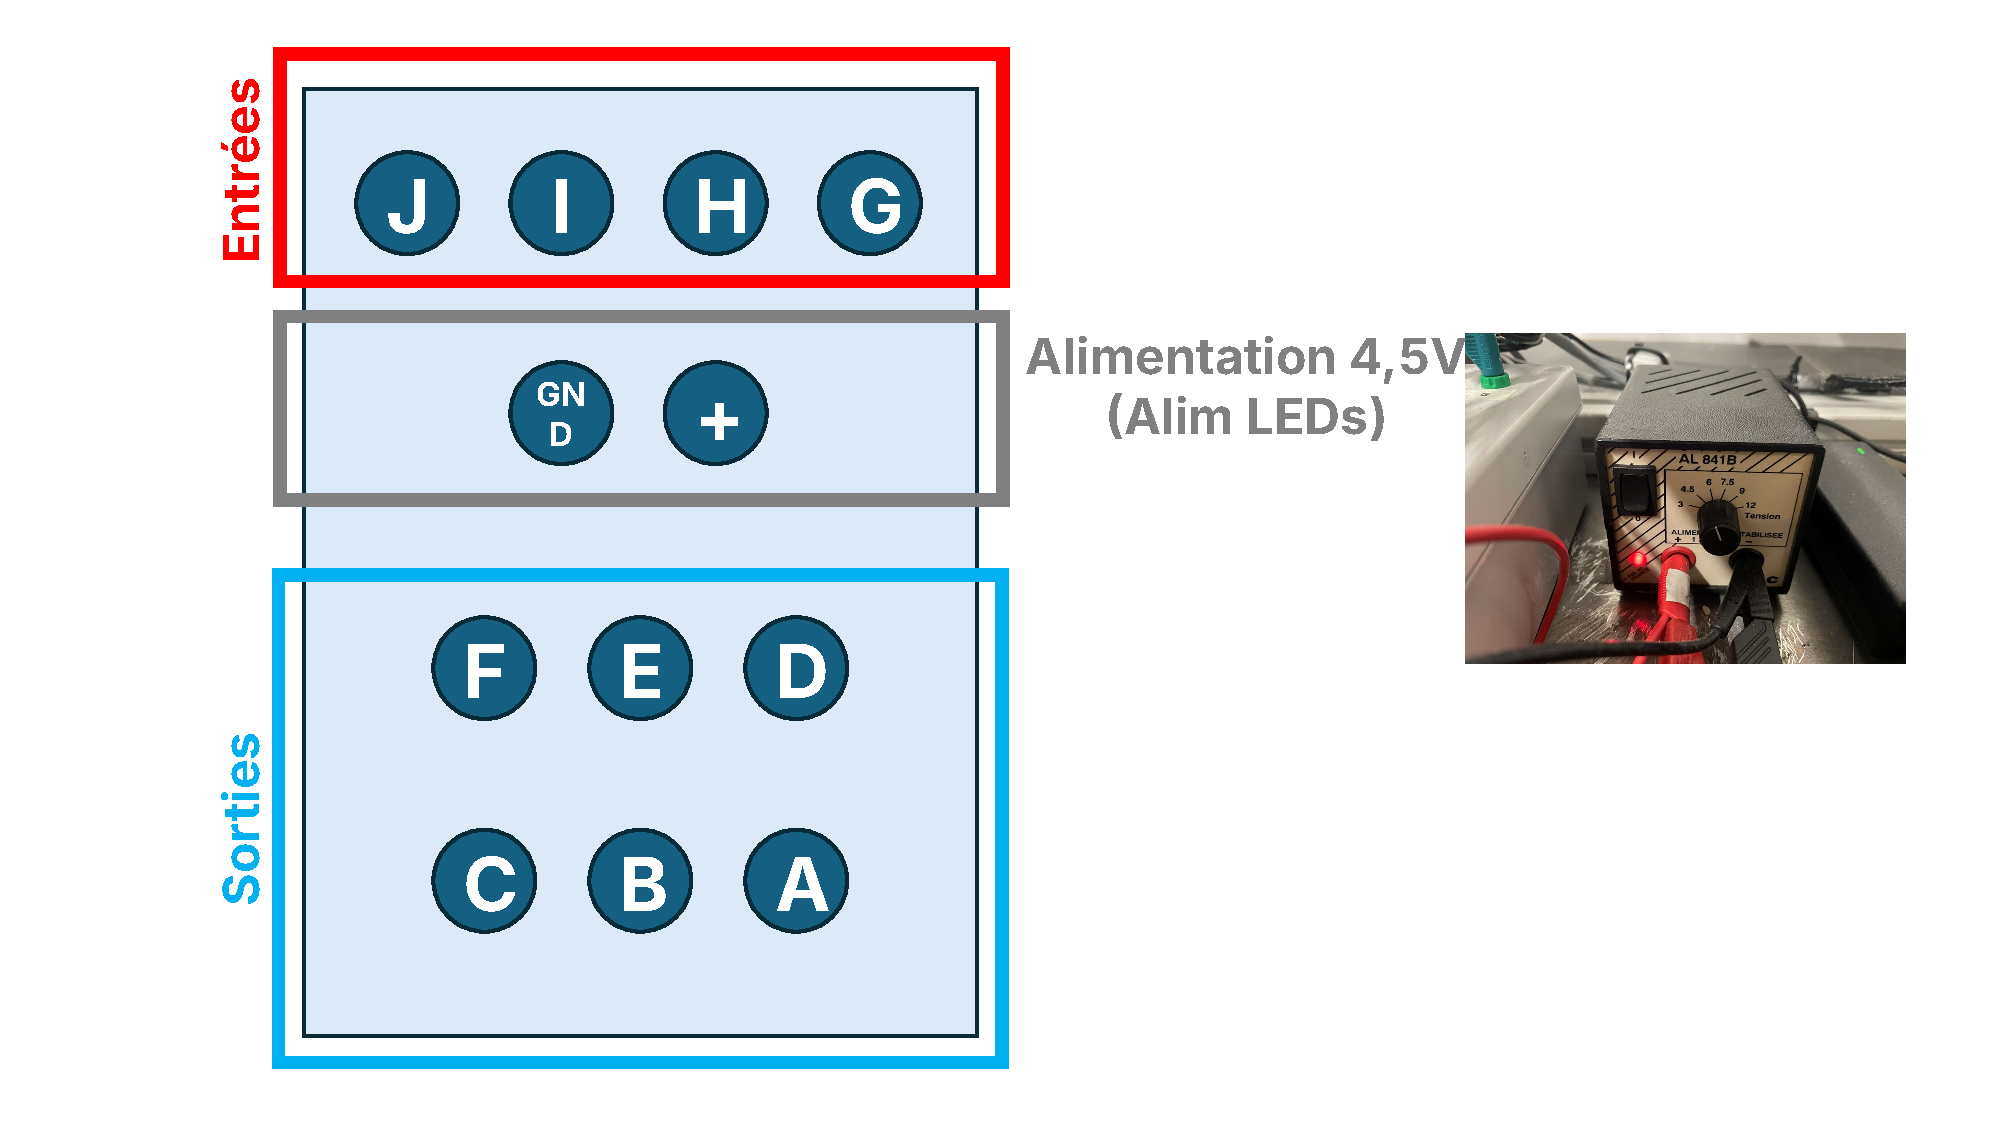
\includegraphics[page=1, width=0.85\textwidth]{images/schemas_relais.pdf}

\scriptsize Face du boîtier : entrées en haut, alimentation au milieu, sorties en bas
\end{frame}

\begin{frame}{Liaisons \lnum{6}, \lnum{7} et \lnum{8} : schéma de principe}
\centering
\resizebox{\textwidth}{!}{%
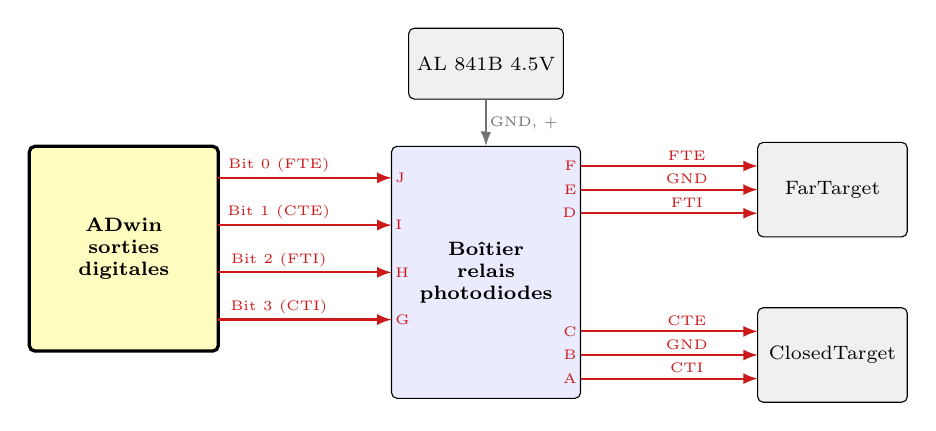
\begin{tikzpicture}
	\node[maitre, minimum width=2.4cm, minimum height=2.6cm] (adwin) at (0,0) {ADwin\\\scriptsize sorties\\\scriptsize digitales};
	\node[appareil, minimum width=2.4cm, minimum height=3.2cm] (boit) at (4.6,-0.3) {};
	\node[font=\scriptsize\bfseries, align=center] at (4.6,-0.3) {Boîtier\\relais\\photodiodes};
	\node[passif, minimum width=1.8cm] (alim) at (4.6,2.35) {AL 841B 4.5V};
	\node[passif, minimum width=1.9cm, minimum height=1.2cm] (ft) at (9.0,0.75) {FarTarget};
	\node[passif, minimum width=1.9cm, minimum height=1.2cm] (ct) at (9.0,-1.35) {ClosedTarget};
	% entrées
	\foreach \b/\l/\s/\y in {0/J/FTE/0.9, 1/I/CTE/0.3, 2/H/FTI/-0.3, 3/G/CTI/-0.9}{
		\draw[lien, cBanane] (1.2,\y) -- node[etiq, above=0.25mm, pos=0.35]{Bit \b\ (\s)} (3.4,\y) node[etiq, right, fill=none]{\l};
	}
	% alimentation
	\draw[lien, cAlim] (alim) -- node[etiq, right]{GND, +} (boit.north);
	% sorties
	\foreach \l/\s/\y in {F/FTE/1.05, E/GND/0.75, D/FTI/0.45}{
		\draw[lien, cBanane] (5.8,\y) node[etiq, left, fill=none]{\l} -- node[etiq, above=0.25mm, pos=0.6]{\s} (8.05,\y);
	}
	\foreach \l/\s/\y in {C/CTE/-1.05, B/GND/-1.35, A/CTI/-1.65}{
		\draw[lien, cBanane] (5.8,\y) node[etiq, left, fill=none]{\l} -- node[etiq, above=0.25mm, pos=0.6]{\s} (8.05,\y);
	}
\end{tikzpicture}}
\end{frame}

\begin{frame}{Liaisons \lnum{6}, \lnum{7} et \lnum{8} : correspondances}
\begin{columns}[t]
\begin{column}{0.5\textwidth}
\begin{block}{\lnum{6} Entrées (ADwin $\rightarrow$ boîtier)}
\centering
\scriptsize
\setlength{\tabcolsep}{3pt}
\begin{tabular}{cll}
	\toprule
	\textbf{Douille} & \textbf{ADwin} & \textbf{Anneau} \\
	\midrule
	G & Bit 3 & ClosedTarget Int. [CTI] \\
	H & Bit 2 & FarTarget Int. [FTI] \\
	I & Bit 1 & ClosedTarget Ext. [CTE] \\
	J & Bit 0 & FarTarget Ext. [FTE] \\
	\bottomrule
\end{tabular}
\end{block}
\begin{block}{\lnum{7} Alimentation}
\scriptsize
AL 841B réglée sur 4.5V $\rightarrow$ douilles GND et +
\end{block}
\end{column}
\begin{column}{0.5\textwidth}
\begin{block}{\lnum{8} Sorties (boîtier $\rightarrow$ cibles)}
\centering
\scriptsize
\begin{tabular}{cl}
	\toprule
	\textbf{Douille} & \textbf{Signal} \\
	\midrule
	A & ClosedTarget Internal [CTI] \\	
	B & Masse (GND) ClosedTarget \\
	C & ClosedTarget External [CTE] \\
	\midrule
	D & FarTarget Internal [FTI] \\
	E & Masse (GND) FarTarget \\
	F & FarTarget External [FTE] \\
	\bottomrule
\end{tabular}
\end{block}
\end{column}
\end{columns}
\end{frame}

%---------------------------------------------------------------------
\subsection{Commande de l'électro-aimant}
\begin{frame}{Liaisons \lnum{9} à \lnum{12} : boîtier relais électro-aimant}
\centering
\includegraphics[page=2, width=0.95\textwidth]{images/schemas_relais.pdf}
\end{frame}

\begin{frame}{Liaisons \lnum{9} à \lnum{12} : schéma de principe}
\centering
\resizebox{\textwidth}{!}{%
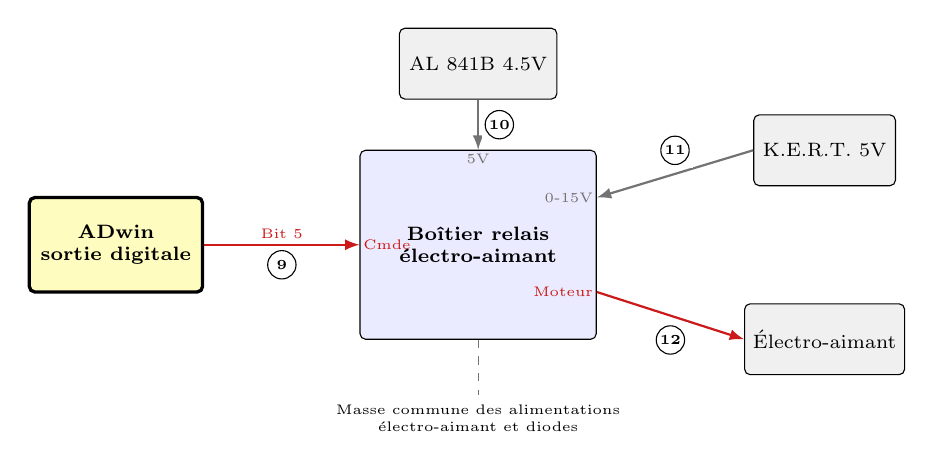
\begin{tikzpicture}
	\node[maitre, minimum width=2.2cm, minimum height=1.2cm] (adwin) at (0,0) {ADwin\\\scriptsize sortie digitale};
	\node[appareil, minimum width=3.0cm, minimum height=2.4cm] (boit) at (4.6,0) {};
	\node[font=\scriptsize\bfseries, align=center] at (4.6,0) {Boîtier relais\\électro-aimant};
	\node[passif, minimum width=2.0cm] (kert) at (4.6,2.3) {AL 841B 4.5V};
	\node[passif, minimum width=1.8cm] (alim) at (9.0,1.2) {K.E.R.T. 5V};
	\node[passif, minimum width=1.8cm] (ea) at (9.0,-1.2) {Électro-aimant};
	\node[font=\tiny, align=center] (gnd) at (4.6,-2.2) {Masse commune des alimentations\\électro-aimant et diodes};

	\draw[lien, cBanane] (adwin) -- node[etiq, above=0.25mm]{Bit 5} node[etiq, below=0.25mm]{\lnum{9}} (boit.west) node[etiq, right, fill=none]{Cmde};
	\draw[lien, cAlim] (kert) -- node[etiq, right=0.4mm]{\lnum{10}} (boit.north) node[etiq, below, fill=none]{5V};
	\draw[lien, cAlim] (alim.west) -- node[etiq, above=0.7mm]{\lnum{11}} ([yshift=6mm]boit.east) node[etiq, left, fill=none]{0-15V};
	\draw[lien, cBanane] ([yshift=-6mm]boit.east) node[etiq, left, fill=none]{Moteur} -- node[etiq, below=0.8mm]{\lnum{12}} (ea.west);
	\draw[dashed, cAlim] (boit.south) -- (gnd.north);
\end{tikzpicture}}
\end{frame}

\begin{frame}{Liaisons \lnum{9} à \lnum{12} : correspondances}
\centering
\footnotesize
\setlength{\tabcolsep}{4pt}
\begin{tabular}{clll}
	\toprule
	\textbf{N°} & \textbf{Douilles du boîtier} & \textbf{Reliées à} & \textbf{Rôle} \\
	\midrule
	9  & Cmde              & ADwin, sortie Bit 5 & Commande du relais \\
	10 & 5V                & Alim. AL 841B (4.5V) & Alimentation du boîtier \\
	11 & 0-15V (haut)      & Alim. K.E.R.T. (5V) & Puissance électro-aimant \\
	12 & Moteur (bas)      & Électro-aimant      & Sortie relais \\
	\bottomrule
\end{tabular}
\vspace{0.5cm}

\begin{alertblock}{Masse}
\justifying
La douille du bas de la colonne centrale (5V) est la masse commune des deux alimentations : électro-aimant et diodes.
\end{alertblock}
\end{frame}

%=====================================================================
\section{Points à définir}
%=====================================================================
\begin{frame}
\begin{block}{Éléments à définir ultérieurement (ADU)}
\begin{itemize}
\justifying
	\item Emplacements définitifs sur le CodaHub des câbles DB25 (trigger) et DB9 (ODIN)
	\item Brochage du câble DB9 ADwin $\rightarrow$ CODAmotion (documentation ODIN)
	\item Photographies du bouton poussoir, des cibles et de l'électro-aimant 
\end{itemize}
\end{block}
\end{frame}

\end{document}
